\documentclass[10pt]{article}

\usepackage[margin=0.78in]{geometry}
\usepackage[T1]{fontenc}
\usepackage{lmodern}
\usepackage{microtype}
\usepackage{amsmath,amssymb}
\usepackage{booktabs}
\usepackage{tabularx}
\usepackage{array}
\usepackage{graphicx}
\usepackage{xcolor}
\usepackage{hyperref}
\usepackage{natbib}
\usepackage{siunitx}
\usepackage{enumitem}
\usepackage{caption}
\usepackage{float}
\usepackage{pdflscape}
\usepackage{tikz}
\usetikzlibrary{arrows.meta,positioning,fit}

\definecolor{ink}{HTML}{172B3A}
\definecolor{accent}{HTML}{176B87}
\definecolor{softblue}{HTML}{EAF3F7}
\definecolor{softgray}{HTML}{F3F5F6}
\hypersetup{
  colorlinks=true,
  linkcolor=accent,
  citecolor=accent,
  urlcolor=accent,
  pdftitle={Expressivity Engineering for Single-Layer Reinforcement Learning},
  pdfauthor={Hanting Wu}
}
\setlist{nosep,leftmargin=1.4em}
\setlength{\parindent}{0pt}
\setlength{\parskip}{0.42em}
\sisetup{detect-all,round-mode=places,round-precision=3}

\newcommand{\EE}{\textit{Expressivity Engineering}}
\newcommand{\TriGLU}{\textsc{TriGLU}}
\newcommand{\ToTGLU}{\textsc{ToTGLU}}
\newcommand{\GRPO}{\textsc{GRPO}}
\newcommand{\ourmodel}{Layer-10 \TriGLU{}}
\newcommand{\baseline}{Layer-10 baseline}
\newcommand{\caveat}[1]{\textcolor{ink}{\textbf{Boundary.} #1}}

\title{\vspace{-1.5em}\textbf{Expressivity Engineering for Single-Layer Reinforcement Learning}\\
\large A Controlled TriGLU Study on Qwen3-1.7B-Base}
\author{Hanting Wu\\\small Independent Research}
\date{July 2026}

\begin{document}
\maketitle

\begin{abstract}
We introduce \EE{} (EE) from a multiplication-first distinction: a static
linear map performs pure channel mixing, whereas multiplying a representation
by itself, or by a transformed version of itself, creates higher-order and
input-conditioned interaction.  Under this lens, nonlinear activation
functions, GLU-family gates, attention, routed MoE/MoLoRA, and HyperNetworks
are not disconnected tricks; they are different realizations of input-derived
multiplication or dynamic weighting.  To test this proposal under a bounded
compute budget, we use the layer-selective reinforcement learning workflow of
\citet{zhang2026onelayer} as experimental guide rails:
Qwen3-1.7B-Base is trained with Group Relative Policy Optimization while only
decoder Layer 10 is updated.  The EE intervention retains the original SwiGLU
path and adds an exact-no-op-initialized, FP32 side network that multiplicatively
modulates the Layer-10 SwiGLU hidden state.  The implementation, called
\TriGLU{} in code and more descriptively \ToTGLU{} in this report, adds
20,986,368 parameters, or 41.69\% of one Qwen3-1.7B decoder layer.

We compare the intervention with a matched naive whole-Layer-10 baseline.  Both
runs start from the same untuned Qwen3-1.7B-Base revision and share data order,
initialization and rollout seeds, reward, response cap, and a six-GPU
\texttt{504/126/6} train/mini/micro-batch contract.  Corrected evaluations are
reported at matched global steps 158, 196, 226, 256, and 294.  Averaged across
these correlated checkpoints, \TriGLU{} improves MathAvg from 52.224 to 52.997
(+0.773 points) and the provisional CodeAvg from 32.671 to 33.659 (+0.988),
while Reasoning and Language category averages are approximately tied
(-0.213 and -0.128).  The clearest gains occur on harder generative tasks:
\textbf{OlympiadBench} (+2.548), \textbf{corrected LiveCodeBench} (+1.063), and a manually
audited \textbf{GPQA-Diamond-Freeform} diagnostic (+1.746).  These results are promising
but not definitive: they come from one training seed, checkpoint variation is
not independent-seed uncertainty, several evaluation protocols required
correction, and response-length caps remain in both training and evaluation.
The study therefore establishes an artifact-backed positive pilot for EE-PEFT, not
a general scaling-law claim.
\end{abstract}

\section{Introduction}

\EE{} begins from one operation: multiplication.  For a representation $x$, a
static linear map $Wx$ performs channel mixing.  It can recombine coordinates,
but a single such map does not create products between input-dependent
features.  Multiplying a representation by itself, or by a learned
preprocessing of itself, changes that algebraic structure.  Expressions such
as $f(x)\odot g(x)$ contain feature products; expressions such as $W(x)x$ use
the current state to construct the weights that act on that same state.  We
take this self- or input-conditioned multiplication, rather than a list of
particular modules, as the primitive of \EE{}.

This primitive reveals a shared structure beneath mechanisms that are usually
placed in separate literatures.  A nonlinear activation can be approximated
over a bounded operating range by polynomial terms, whose powers are repeated
self-multiplications.  GLU and SwiGLU multiply learned feature streams
\citep{shazeer2020glu}.  Attention constructs an input-dependent weight matrix
from queries and keys and multiplies it into values
\citep{vaswani2017attention}.  HyperNetworks generate the parameters that act
on another representation \citep{ha2016hypernetworks}.  MoE and MoLoRA multiply
expert outputs by routed, input-dependent coefficients
\citep{shazeer2017moe,zadouri2024molora}.  These are not mathematically
identical modules, but they instantiate the same engineering move: replace
only fixed linear channel mixing with computation whose effective transform is
conditioned on, and multiplied with, the current representation.

We propose \EE{} as a unifying engineering lens for this move.  It is a working
taxonomy rather than a theorem that totally orders neural architectures by
expressive power.  It is useful because it separates two questions:

\begin{enumerate}
  \item How much additional input-dependent interaction is introduced?
  \item Where can that interaction be inserted and trained economically?
\end{enumerate}

The present study addresses the second question through layer-selective RL.
\citet{zhang2026onelayer} show that RL gains in Qwen3 and related models are
concentrated in a small set of middle layers; on Qwen3-1.7B-Base, Layer 10 is
their strongest single-layer math result.  That finding is not the conceptual
origin of EE.  It supplies the empirical localization result and workflow
guide rails that make a compute-bounded test of our independently proposed EE
hypothesis feasible: instead of pretraining a new architecture from scratch,
we can add expressivity at one high-contribution layer and compare it against a
naive update of exactly the same layer.

Our contributions are:

\begin{itemize}
  \item a multiplication-first EE taxonomy connecting general nonlinear
        activations, GLU-family FFNs, attention, HyperNetworks, routed full and
        low-rank experts, grid-wise modulation, and explicit polynomial
        modules;
  \item an exact-function-preserving Layer-10 \TriGLU{}/\ToTGLU{} intervention
        for Qwen3-1.7B-Base;
  \item a matched six-GPU GRPO comparison from the same untuned base model,
        with deterministic data exposure and five common evaluation
        checkpoints;
  \item corrected Math and out-of-distribution evaluation records, including a
        strict free-form GPQA-Diamond audit and explicit protocol/cap-hit
        boundaries;
  \item a systems account of registered Hugging Face/vLLM integration,
        continuous batching, live weight synchronization, and the current
        serving-performance cost of the FP32 side branch.
\end{itemize}

\section{Expressivity Engineering}

\subsection{A working definition}

For an input vector $x$, the baseline operation is fixed linear channel mixing,
$y=Wx$.  The defining EE move is instead to multiply an input-derived quantity
back into the same representation or into another transform of it:
\begin{equation}
  y = f(x) \odot g(x)
  \quad\text{or}\quad
  y = W(x)x.
  \label{eq:ee-primitive}
\end{equation}
The first form includes literal self-interaction when $f=g$, and interaction
with a preprocessed self when $f$ and $g$ are different transforms of the same
input.  The second is the matrix-valued version: $x$ generates some or all of
the weights that are then applied to $x$.  Familiar mechanisms can be written
as instances of these forms:
\begin{align}
  \text{activation:}\quad
    &\phi(z) \approx \sum_{k=0}^{K} a_k z^{\odot k},
    \label{eq:ee-activation}\\
  \text{GLU:}\quad
    &y = \phi(Ax) \odot Bx,
    \label{eq:ee-glu}\\
  \text{attention:}\quad
    &Y = \operatorname{softmax}\!\left(\frac{Q(X)K(X)^\top}{\sqrt{d}}\right)V(X),
    \label{eq:ee-attention}\\
  \text{dynamic weights:}\quad
    &y = \left(W + \Delta W(x)\right)x,
    \label{eq:ee-hyper}\\
  \text{routed experts:}\quad
    &y = \sum_e \pi_e(x) f_e(x).
  \label{eq:ee-family}
\end{align}
Equation~\ref{eq:ee-activation} is an approximation statement on a bounded
domain, not a claim that every activation is globally polynomial.  It makes
the key algebraic point: nonlinear activation functions introduce powers and
self-interactions that a lone linear channel mixer cannot.  GELU, for example,
is explicitly $z\Phi(z)$ \citep{hendrycks2016gelu}; PolyCom/PolyNorm makes the
polynomial view trainable and explicit \citep{zhuo2024polycom}.  Under this
definition:

\begin{itemize}
  \item general nonlinear activations are the most local form of EE: they turn
        each channel into a nonlinear self-interaction before later channel
        mixing; explicit polynomial activations expose this structure rather
        than creating it from nothing;
  \item GLU/SwiGLU makes the multiplication visible by gating one learned
        stream with another \citep{shazeer2020glu};
  \item attention is dynamic weighting at token level: $Q(X)$ and $K(X)$
        construct weights from the current sequence, and those weights
        multiply $V(X)$ \citep{vaswani2017attention};
  \item HyperNetworks generate parameters for another network
        \citep{ha2016hypernetworks};
  \item HyperGrid decomposes task-conditioned modulation into grid-wise
        projections \citep{tay2020hypergrid};
  \item HyperFormer generates task/layer/position-conditioned adapter
        parameters, and HyperLoRA generates constrained low-rank adapters
        \citep{mahabadi2021hyperformer,lv2024hyperlora};
  \item MoE multiplies full expert outputs by router coefficients
        \citep{shazeer2017moe}, while MoLoRA applies the same routed-mixture
        pattern to low-rank updates \citep{zadouri2024molora}.  At the routing
        level, a conventional linear-logit MoE router is the full-expert
        analogue of linearly routed MoLoRA; their expert parameterizations,
        capacities, and compute profiles remain different;
  \item PolyCom/PolyNorm makes higher-order activation interactions explicit
        and trainable \citep{zhuo2024polycom}.
\end{itemize}

The claim is common primitive, not module equivalence.  HyperFormer and
HyperLoRA are primarily task-conditioned parameter generators; attention is a
per-token dynamic weight matrix over values; MoE routes among full experts;
MoLoRA routes among low-rank updates; HyperGrid modulates structured regions of
weight matrices; and PolyNorm uses elementwise polynomial powers and
normalization.  The present \TriGLU{} branch is another point in this family:
it computes a per-token multiplicative modulation of one existing FFN hidden
state.

\subsection{Scope beyond Transformers}

The EE lens is not limited to language models.  Any architecture containing an
MLP can, in principle, be augmented with multiplicative, routed, polynomial, or
dynamically parameterized computation.  For Transformer FFNs, such operations
remain linear in sequence length, unlike dense self-attention's quadratic
token-pair interaction.  This does not make EE free: added FFN branches increase
FLOPs, activation memory, kernel-launch overhead, and optimization difficulty.
It does mean that richer channel computation can be explored without directly
increasing the number of attention score pairs or the KV-cache length.

Attention is therefore not merely adjacent background; it is a canonical EE
mechanism at token-mixing scale.  Its effective matrix
$\operatorname{softmax}(QK^\top/\sqrt{d})$ is generated from the current hidden
states before it weights the values.  This controlled study nevertheless keeps
the attention architecture unchanged: only the Layer-10 FFN computation
differs between conditions, while the ordinary Layer-10 attention parameters
remain trainable in both.  The experiment tests whether the same broad
multiplication-first principle can be pushed further inside the FFN without
changing attention.

\section{Model}

\subsection{Backbone and update scope}
\label{sec:backbone-scope}

The backbone is Qwen3-1.7B-Base \citep{yang2025qwen3}: 28 decoder layers,
hidden width 2,048, FFN intermediate width 6,144, 16 query heads, 8 key/value
heads, and a 32,768-token context window.  Both the baseline and EE variant
update decoder Layer 10 only.  Layer-10 attention projections, RMSNorm
parameters, and all original FFN projections are trainable.  Embeddings, the
language-model head, and all other decoder layers are frozen.

This is a stricter comparison than using the untuned base model as the primary
control.  The question is not whether RL helps, but whether adding a particular
expressivity mechanism improves a strong naive single-layer RL update.

\subsection{TriGLU/ToTGLU side modulation}

Let $x\in\mathbb{R}^{2048}$ be the Layer-10 FFN input.  The original SwiGLU
hidden state is
\begin{equation}
  h_0 = \operatorname{SiLU}(W_g x) \odot (W_u x),
  \qquad h_0\in\mathbb{R}^{6144}.
\end{equation}
The FP32 side network first compresses to a 512-dimensional bottleneck,
$z=A x\in\mathbb{R}^{512}$, and forms three 2,048-dimensional streams:
\begin{align}
  v &= Vz, \\
  g &= \operatorname{SiLU}(Gz), \\
  q &= \operatorname{SiLU}\!\left(F_2\operatorname{GeLU}(F_1z)\right).
\end{align}
Their product is projected to the backbone intermediate width,
\begin{equation}
  s = U(v\odot g\odot q)\in\mathbb{R}^{6144},
\end{equation}
and modulates the original hidden state:
\begin{equation}
  h = h_0 \odot \left[1 + \alpha\tanh(s)\right],
  \qquad
  y = W_d h,
  \qquad \alpha=0.1.
  \label{eq:triglu}
\end{equation}

The code calls this module \TriGLU{}.  Because the base SwiGLU already contains
two multiplicative streams and the side branch multiplies three more, we use
\ToTGLU{} (``TriGLU on TriGLU'') when emphasizing its five-stream
interpretation.  The name is descriptive rather than a claim that the module
implements a standard architecture from prior work.

\begin{figure}[H]
\centering
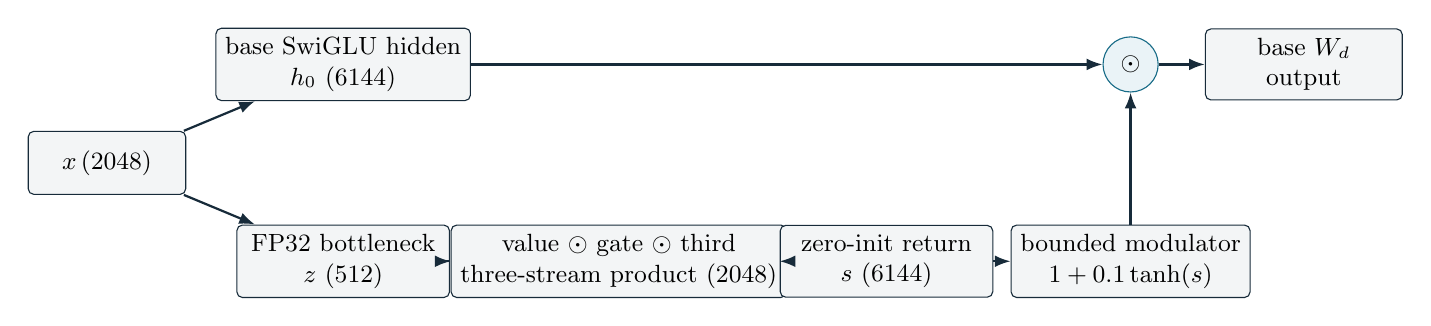
\begin{tikzpicture}[
  x=1cm,y=1cm,
  box/.style={draw=ink,rounded corners=2pt,fill=softgray,minimum height=8mm,align=center,font=\small},
  op/.style={draw=accent,circle,fill=softblue,minimum size=7mm,font=\small\bfseries},
  arr/.style={-{Latex[length=2mm]},thick,draw=ink}
]
\node[box,minimum width=20mm] (x) at (0,0) {$x$\,(2048)};
\node[box,minimum width=27mm] (base) at (3.0,1.25) {base SwiGLU hidden\\$h_0$ (6144)};
\node[box,minimum width=27mm] (bneck) at (3.0,-1.25) {FP32 bottleneck\\$z$ (512)};
\node[box,minimum width=34mm] (three) at (6.5,-1.25) {value $\odot$ gate $\odot$ third\\three-stream product (2048)};
\node[box,minimum width=27mm] (side) at (9.9,-1.25) {zero-init return\\$s$ (6144)};
\node[box,minimum width=29mm] (mod) at (13.0,-1.25) {bounded modulator\\$1+0.1\tanh(s)$};
\node[op] (mul) at (13.0,1.25) {$\odot$};
\node[box,minimum width=25mm] (down) at (15.2,1.25) {base $W_d$\\output};
\draw[arr] (x) -- (base);
\draw[arr] (x) -- (bneck);
\draw[arr] (bneck) -- (three);
\draw[arr] (three) -- (side);
\draw[arr] (side) -- (mod);
\draw[arr] (base) -- (mul);
\draw[arr] (mod) -- (mul);
\draw[arr] (mul) -- (down);
\end{tikzpicture}
\caption{Layer-10 \TriGLU{}/\ToTGLU{} intervention.  The original SwiGLU path
is retained.  A per-token FP32 side network produces a bounded multiplicative
modulator before the original down projection.}
\label{fig:architecture}
\end{figure}

\subsection{Exact no-op initialization and parameter cost}

The side return projection $U$ (named \texttt{triglu\_side.up} in code) is
initialized to zero.  Therefore $s=0$, the multiplier in
Eq.~\ref{eq:triglu} is exactly one, and the initial model is functionally
identical to the unmodified backbone.  This invariant isolates subsequent
behavior from a random architecture shock.

The active dimensions are \texttt{side\_dim=512} and
\texttt{side\_hidden=2048}.  The side network contains 20,986,368 trainable
parameters, 41.69\% of the 50,337,792-parameter selected decoder layer.  The
base Layer-10 parameters remain jointly trainable.  This is parameter-efficient
relative to full-model RL, but it is deliberately a high-capacity intervention
rather than a minimal adapter.

\section{Experimental Design}

\subsection{Relationship to the layer-selective RL workflow}
\label{sec:layer-selective-workflow}

The experiment follows the operational structure of
\citet{zhang2026onelayer}: Qwen3-1.7B-Base, Layer 10, NuminaMath-CoT, GRPO,
single-layer freezing, a 3,072-token response cap, and Math plus OOD benchmark
families.  The original work reports that Layer 10 reaches 51.8 MathAvg versus
50.8 for full-parameter RL under its protocol.  Its results and hyperparameters
are guide rails, not copied output: its executable repository and exact
evaluation harness were not available to this study, so absolute score parity
is not claimed.

Our scientific variable is the Layer-10 FFN architecture.  The baseline updates
the ordinary Layer-10 Transformer block; the EE condition updates that same
block plus the side network.  Both begin from the same untuned base model.

\subsection{Data and decontamination}

Training uses a 50,000-problem materialization derived from NuminaMath-CoT
\citep{numina2024}.  A decontamination pass removes question-level overlap with
the evaluation sets before training.  The two variants use the same parquet
hashes, deterministic shuffled permutation, omitted-row set, initialization
seed, and rollout seed (\texttt{20260707}).  This controls data exposure within
the comparison; it does not prove that the local data processing exactly
matches an unavailable external implementation.

\subsection{GRPO and the six-GPU batch contract}

GRPO samples a group of responses per prompt and normalizes their advantages
within the group, avoiding a learned critic \citep{shao2024deepseekmath}.  The
implementation uses veRL/HybridFlow \citep{sheng2025hybridflow} with vLLM
rollouts \citep{kwon2023vllm}.  The paper-aligned tuple is train/mini/micro
batch \texttt{512/128/8}, group size 4, KL coefficient 0.001, clip range 0.2,
and four epochs.  The actual six-RTX-5090 matched run uses the explicitly
approved divisible tuple in Table~\ref{tab:batch}.

\begin{table}[!tbp]
\centering
\caption{Six-rank production contract.}
\label{tab:batch}
\begin{tabular}{lr}
\toprule
Field & Value \\
\midrule
Train batch & 504 prompts \\
PPO mini batch & 126 prompts \\
PPO micro batch & 6 prompts \\
Group size & 4 responses/prompt \\
Responses per global update & 2,016 \\
Prompts through step 98 & 49,392 \\
Deterministically omitted at step 98 & 608 / 50,000 \\
Rollout replicas & 6 independent TP=1 replicas \\
\bottomrule
\end{tabular}
\end{table}

The loader uses \texttt{drop\_last=True}; step 98 is therefore a
\emph{near-one-pass} milestone, not an exact epoch.  No irregular tail batch is
introduced.  Both architectures omit exactly the same 608 rows, giving a
matched comparison with a 1.56\% exposure deviation from $512\times98$.

\subsection{Training stages and post-hoc interventions}

The trajectory contains three 98-update stages.  The first uses the original
$5\times10^{-6}$ learning rate.  The second keeps that rate through step 128
and then applies cosine decay to $5\times10^{-7}$ at step 196.  The third
decays from $5\times10^{-7}$ to $5\times10^{-8}$ at step 294.  Each variant's
frozen KL reference is reset to its own step-98 policy for updates 99--196 and
to its own step-196 policy for updates 197--294.

The decay and reference resets were introduced during the live research cycle,
not preregistered before update 1.  Step 158 is the first reported common
checkpoint after the step-128 schedule change and the first point where the
architectural trajectories visibly separated.  We report all available matched
major checkpoints from 158 onward rather than selecting a single best model.

\subsection{Historical SFT pilot}

Before the main RL wave, a two-epoch, 50K-example supervised fine-tuning pilot
compared SHS, the whole-layer baseline, \TriGLU{}, and OFT.  It completed
operationally, but did not provide a reliable architecture selection signal.
SHS, baseline, and \TriGLU{} had four-task Math averages within 0.32 points.
OFT achieved the lowest teacher-forced validation loss (0.5893) yet collapsed
under autoregressive evaluation (13.04 Math average versus approximately 43
for the other three).  This is direct evidence in this project that
same-distribution SFT loss is not a sufficient proxy for the intended
generative reasoning behavior.  Consequently, the main GRPO comparison starts
from the untuned base, not from an SFT checkpoint.

OFT \citep{qiu2023oft} was scaffolded but not run as a GRPO comparator.  The
implemented policy freezes the original Layer-10 SwiGLU matrices and trains
orthogonal rotations, whereas \TriGLU{} jointly trains the original SwiGLU and
the side branch.  A direct comparison would therefore confound architectural
expressivity with different backbone adaptation constraints.  OFT remains a
useful future control under a matched update policy.

\section{Evaluation}

\subsection{Benchmark suite and aggregate definitions}

The in-domain Math category follows MATH-500 \citep{hendrycks2021math}, GSM8K
\citep{cobbe2021gsm8k}, OlympiadBench \citep{he2024olympiadbench}, and the
2023 AMC 10/12 competition set \citep{maa2023amc}.  MathAvg is the unweighted
mean of those four scores and uses AMC
Average@32, not AMC greedy pass@1.  AMC greedy is retained as a modal-path
diagnostic.

OOD evaluation includes:
\begin{itemize}
  \item Code: corrected HumanEval+ \citep{liu2023evalplus}, provisional MBPP
        \citep{austin2021mbpp}, and corrected LiveCodeBench
        \citep{jain2024livecodebench};
  \item Reasoning: GPQA-Diamond \citep{rein2023gpqa} and MMLU-Pro
        \citep{wang2024mmlupro}, plus a separate GPQA-Diamond-Freeform manual
        diagnostic that is not included in ReasoningAvg;
  \item Language and instruction following: C-Eval \citep{huang2023ceval},
        IFEval \citep{zhou2023ifeval}, and MGSM \citep{shi2022mgsm}.
\end{itemize}

Except AMC Average@32, the primary corrected benchmark cells use greedy
decoding.  This choice is especially important for the FP32 \TriGLU{} model,
whose sampled generations at temperature 1 were less stable.  The report does
not convert that observation into a deployment recommendation; temperature
and logit-distillation behavior require a dedicated study.

\subsection{Benchmark semantics and relative difficulty}

The suite intentionally spans different capability regimes.  ``Difficulty''
below is a qualitative task-level description, not a claim that scores are
directly comparable across datasets.

\begin{table}[H]
\centering
\small
\caption{Benchmark roles in the evaluation suite.}
\label{tab:benchmarkroles}
\begin{tabularx}{\linewidth}{>{\raggedright\arraybackslash}p{0.19\linewidth}
                             >{\raggedright\arraybackslash}p{0.43\linewidth}
                             >{\raggedright\arraybackslash}X}
\toprule
Benchmark & Task and answer format & Relative regime \\
\midrule
MATH-500 & Competition-style secondary mathematics; free-form numeric or symbolic answer & Harder than routine school arithmetic; broad algebra, geometry, number theory, and combinatorics \\
GSM8K & Grade-school arithmetic word problems; free-form short answer & Elementary mathematics with multi-step linguistic reasoning \\
OlympiadBench & Olympiad-oriented mathematics; free-form derivation and answer & Hardest in-domain mathematical set in this report \\
AMC 2023 & AMC 10/12 high-school contest questions; multiple choice & Between routine K--12 work and olympiad-style proof problems \\
HumanEval+ & Function synthesis from a specification; execution-based tests & Compact code generation with strengthened hidden tests \\
MBPP & Short natural-language programming tasks; execution-based tests & Introductory-to-intermediate code generation; score remains provisional here \\
LiveCodeBench & Time-indexed competitive-programming problems; execution-based tests & Harder and less contamination-prone coding evaluation \\
GPQA-Diamond & Graduate-level science questions; four-way multiple choice & Expert factual and scientific reasoning; 25\% random-choice floor \\
MMLU-Pro & Ten-choice, multi-domain knowledge and reasoning & Broad professional/academic reasoning with a 10\% random-choice floor \\
GPQA-Diamond-Freeform & Same science questions without answer options; manual semantic audit & Stricter diagnostic that removes the multiple-choice floor \\
C-Eval & Chinese multi-subject multiple choice & Broad school-to-professional knowledge in Chinese \\
IFEval & Verifiable instruction-following constraints & Tests compliance rather than subject-matter depth \\
MGSM & Multilingual grade-school mathematics; free-form short answer & Elementary mathematics under cross-lingual generation pressure \\
\bottomrule
\end{tabularx}
\end{table}

\subsection{Protocol corrections}

Several legacy evaluation cells measured harness failures rather than model
capability.  The corrected table therefore uses:
\begin{itemize}
  \item a raw no-chat HumanEval+ route after the chat-wrapped protocol caused
        Hebrew/template collapse in both \TriGLU{} and the untuned base;
  \item a corrected LiveCodeBench sandbox output contract after the legacy
        contract produced an artificial all-zero result;
  \item explicit separation of AMC Average@32 from greedy pass@1;
  \item a row-by-row semantic audit of 1,260 GPQA-Diamond-Freeform responses,
        with uncertain judgments counted as incorrect.
\end{itemize}

These corrections preserve prompts and scoring intent, but do not establish
paper-exact evaluation parity.  MBPP still lacks a full protocol-matrix rerun;
its score and the derived CodeAvg remain provisional.

\subsection{Response-cap boundary}

All Math benchmarks contain 3,072-token cap hits: 5.02\% on MATH-500, 0.43\%
on GSM8K, 13.85\% on OlympiadBench, 3.84\% on AMC Average@32, and 8.25\% on
AMC greedy.  Training rollouts also contain nonzero cap hits.  Many inspected
cases are repetition loops, but a minority could conceivably reach a correct
answer if continued.  We retain the paper-style cap-hit-inclusive results for
matched comparison and do not describe them as uncapped capability ceilings.

OOD cap rates are more heterogeneous.  HumanEval+ is 2.50\%, LiveCodeBench
9.73\%, GPQA-Diamond 9.85\%, MMLU-Pro 4.73\%, MGSM 8.61\%, and
GPQA-Diamond-Freeform 7.62\%.  MBPP (93.92\%), C-Eval (68.31\%), and IFEval
(39.09\%) are severe exceptions that require protocol-aware reruns before
strong absolute interpretation.

\section{Results}

\subsection{Across-checkpoint summary}

\textbf{Table~\ref{tab:means} reports the population mean and standard
deviation across five matched late-stage checkpoints, not across independent
training seeds.}  An independent multiple-seed sweep was outside the available
compute budget: the study had six RTX 5090 GPUs and was scoped to days rather
than weeks.  The checkpoints were therefore drawn from the regime in which both
training reward and downstream evaluation had plateaued and then oscillated
rather than exhibiting a sustained trend.  They sample local within-run
variability from one seeded realization of the stochastic training process,
including shuffled data order and rollout sampling.  Because they belong to one
optimization trajectory, the observations are serially dependent and may be
positively correlated.  This dependence does not invalidate their mean as a
descriptive summary that reduces sensitivity to choosing one favorable
checkpoint, but it lowers the effective sample size: the reported standard
deviation measures checkpoint variation, not independent-seed uncertainty, a
standard error, or a confidence interval.

This summary is operationally relevant because production model selection
normally chooses the better validated checkpoint from a late-stage candidate
pool rather than blindly deploying the final update.  The across-checkpoint
mean characterizes the average quality available within that selection window,
and the per-checkpoint record shows the candidates from which a deployment
choice can be made.  It does not imply that every checkpoint is equally strong:
the magnitude and even direction of the \TriGLU{}--baseline difference vary by
checkpoint, and the benchmarks showing the most prominent gains are not
identical at every checkpoint.

\begin{table}[H]
\centering
\caption{Corrected matched-checkpoint results (steps 158/196/226/256/294).
Values are mean $\pm$ population standard deviation in percentage points.
$^*$MBPP and therefore CodeAvg remain provisional.  $^\dagger$All category
averages are equal-weight descriptive summaries and are intentionally muted;
the three bold rows are the hard generative benchmarks discussed in the text.
\textbf{``Baseline'' denotes the best layer from the source single-layer
reinforcement-learning (SLRL) study---Layer 10---not the untuned base model and
not full-parameter RL.  A
negative difference therefore means only that \TriGLU{} trails this strongest
SLRL comparator on that metric; it does not establish fundamental capability
degradation below the untuned base.  The source protocol reports Layer-10 SLRL
at 51.8 MathAvg versus 50.8 for full-parameter RL, so parity or a small deficit
relative to this baseline may still correspond to parity or an improvement
relative to full RL, subject to the cross-harness boundary in
Sections~\ref{sec:backbone-scope} and \ref{sec:layer-selective-workflow}.}}
\label{tab:means}
\small
\begin{tabular}{lrrr}
\toprule
Metric & \TriGLU{} & Baseline & Mean difference \\
\midrule
MATH-500 & $67.520\pm1.230$ & $66.880\pm0.412$ & $+0.640$ \\
GSM8K & $82.942\pm0.322$ & $82.396\pm0.446$ & $+0.546$ \\
\textbf{OlympiadBench} & $\mathbf{28.059\pm1.294}$ & $\mathbf{25.511\pm0.533}$ & $\mathbf{+2.548}$ \\
AMC 2023 Average@32 & $33.469\pm0.755$ & $34.109\pm0.950$ & $-0.640$ \\
\textcolor{gray}{MathAvg$^\dagger$} & \textcolor{gray}{$52.997\pm0.184$} & \textcolor{gray}{$52.224\pm0.393$} & \textcolor{gray}{$+0.773$} \\
AMC 2023 greedy & $38.000\pm1.000$ & $35.500\pm2.915$ & $+2.500$ \\
\midrule
HumanEval+ corrected & $60.854\pm0.896$ & $59.512\pm1.131$ & $+1.342$ \\
MBPP$^*$ & $29.280\pm1.121$ & $28.720\pm0.844$ & $+0.560$ \\
\textbf{LiveCodeBench corrected} & $\mathbf{10.845\pm0.401}$ & $\mathbf{9.782\pm0.139}$ & $\mathbf{+1.063}$ \\
\textcolor{gray}{CodeAvg$^{*\dagger}$} & \textcolor{gray}{$33.659\pm0.260$} & \textcolor{gray}{$32.671\pm0.567$} & \textcolor{gray}{$+0.988$} \\
\midrule
GPQA-Diamond (MCQ) & $26.566\pm1.880$ & $26.565\pm2.273$ & $+0.001$ \\
MMLU-Pro & $33.895\pm0.576$ & $34.320\pm0.198$ & $-0.425$ \\
\textcolor{gray}{ReasoningAvg$^\dagger$} & \textcolor{gray}{$30.230\pm0.691$} & \textcolor{gray}{$30.443\pm1.121$} & \textcolor{gray}{$-0.213$} \\
\textbf{GPQA-Diamond-Freeform} & $\mathbf{6.349\pm1.328}$ & $\mathbf{4.603\pm1.053}$ & $\mathbf{+1.746}$ \\
\midrule
C-Eval & $47.548\pm0.566$ & $46.182\pm0.560$ & $+1.366$ \\
IFEval & $27.421\pm0.669$ & $26.752\pm0.657$ & $+0.669$ \\
MGSM & $56.538\pm5.340$ & $58.960\pm0.199$ & $-2.422$ \\
\textcolor{gray}{LanguageAvg$^\dagger$} & \textcolor{gray}{$43.836\pm1.724$} & \textcolor{gray}{$43.964\pm0.334$} & \textcolor{gray}{$-0.128$} \\
\bottomrule
\end{tabular}
\end{table}

\subsection{What the result supports}

The primary Math result is positive: \TriGLU{} improves MathAvg by 0.773
points across the five matched checkpoints.  The gain is not uniform.  It is
largest on \textbf{OlympiadBench} and is accompanied by positive MATH-500 and GSM8K
differences, while AMC Average@32 is lower.  The separate greedy AMC diagnostic
favors \TriGLU{} by 2.5 points, illustrating that sampled distribution-wide
reliability and the greedy modal path need not move together.

The OOD profile is also structured rather than uniformly positive.  Corrected
HumanEval+ and \textbf{LiveCodeBench} favor \TriGLU{}, with the largest relative coding
gain on the harder \textbf{LiveCodeBench} task.  GPQA-Diamond MCQ is effectively tied,
MMLU-Pro slightly favors the baseline, and strict
\textbf{GPQA-Diamond-Freeform} favors
\TriGLU{}.  C-Eval and IFEval improve, but a large MGSM deterioration at
step 294 creates high \TriGLU{} variance and removes the category-average gain.
The source guide's intuition---extra expressivity may improve hard reasoning
while occasionally destabilizing simpler knowledge retrieval or multilingual
behavior---is consistent with this profile, but is not uniquely established by
it.

These local deficits are relative to the strongest source-selected SLRL layer,
not to the untuned base model.  The broader experiment is an RL improvement over
that starting model; a negative \TriGLU{}--baseline cell therefore does not show
that EE destroyed the underlying capability.  One plausible transfer-specific
hypothesis is that the newly initialized EE path received math RL but no
broad-domain pretraining, so it can trail the best SLRL comparator on isolated
OOD tasks even while improving over the untuned starting point overall.  A
same-harness per-benchmark base comparison and the staged EE-only warm start in
Appendix~\ref{app:followup-agenda} are needed to test that interpretation.

The OOD category averages should therefore be treated as deliberately weak
summaries.  They assign equal weight to benchmarks with different domains,
answer formats, random-choice floors, sample counts, and protocol maturity.
Such an average can hide a gain on a strict generative diagnostic---most clearly
\textbf{GPQA-Diamond-Freeform} here---behind a small loss on an unrelated constituent.
The raw benchmark vector, protocol status, and cross-checkpoint stability are
more informative than the sign of a single unweighted OOD average.

The \textbf{GPQA-Diamond-Freeform} table cell is computed from checkpoint-level strict
accuracy.  Each of the five checkpoints contributes 126 manually audited
responses; uncertain judgments count as incorrect.  Averaging those five
equal-denominator accuracies is equivalent to 40 correct checkpoint--question
runs out of 630 for \TriGLU{} (6.349\%) and 29 out of 630 for the baseline
(4.603\%).  A separate union diagnostic asks how many distinct questions were
solved by at least one checkpoint: 18 of 126 for \TriGLU{} and 12 of 126 for
the baseline.  That union statistic is useful for capability coverage but is
not the value reported in Table~\ref{tab:means}.

This caution is also consistent with the source paper's Qwen3-1.7B layer sweep:
Layer 10 is selected for strong Math contribution, but it is not uniformly the
best layer across OOD categories \citep{zhang2026onelayer}.  One plausible
interpretation is that functional specialization remains relatively diffuse at
this parameter scale, so a mathematically high-contribution layer can still
produce heterogeneous transfer.  The stronger layer-role separation suggested
by larger-model results is a cross-scale hypothesis, not something established
by the present single-seed Qwen3-1.7B experiment.

Training reward and downstream evaluation were not monotonically aligned.  At
several checkpoints the EE variant reached equal or lower recent reward while
obtaining stronger held-out metrics.  This is evidence against selecting these
models by training reward alone.  It does not show that lower reward causes
better generalization; reward sampling, shuffled-batch composition, KL
reference resets, and schedule changes all vary along the same trajectory.

\subsection{Why checkpoint averaging is used}

From step 158 onward, both variants occupy an oscillatory plateau: different
shuffled batches pull the model toward different capability profiles.  In a
production workflow, researchers often select a checkpoint during such a
plateau.  Averaging matched checkpoints therefore reduces dependence on one
post-hoc checkpoint choice and describes the typical observed trajectory.
However, five checkpoints from one run are not five independent experiments.
No claim of statistical significance is made, and a multiple-seed replication
is the most important missing validation.

\subsection{Full corrected checkpoint table}

Table~\ref{tab:mastertable} provides the complete per-checkpoint record.  The
native LaTeX table is generated from the repository's machine-readable consolidated table;
it excludes SFT, untuned-base, and early RL checkpoints by design.  The
report-specific renderer mutes every equal-weight Avg column and emphasizes
\textbf{OlympiadBench}, \textbf{LiveCodeBench}, and
\textbf{GPQA-Diamond-Freeform}; this visual hierarchy
is presentation metadata, not a change to any score.

The body contains ten matched cells: five checkpoints for \TriGLU{} and five
for the baseline.  The final rows report the population mean and standard
deviation across checkpoints within each trajectory.  These are descriptive
trajectory summaries rather than multi-seed confidence estimates.

All displayed values use the corrected protocol where a correction was
available.  HumanEval+ uses the raw no-chat route, and LiveCodeBench uses the
repaired execution contract.  MBPP and its dependent CodeAvg remain marked
provisional because their full protocol matrix is incomplete.  MathAvg is
computed from MATH-500, GSM8K, OlympiadBench, and AMC Average@32; the adjacent
AMC greedy column is intentionally outside that aggregate.  Likewise,
GPQA-Diamond-Freeform is shown beside ReasoningAvg but is excluded from it.
The table retains response-cap-inclusive values, so it should be read together
with Section~5.4 rather than as an uncapped capability ceiling.

\clearpage
\begin{landscape}
\begin{table}[H]
\centering
\caption{Full corrected Math and OOD results at matched RL steps 158, 196,
226, 256, and 294, including across-checkpoint means and population standard
deviations.  MathAvg uses AMC Average@32, not AMC greedy.  ReasoningAvg excludes
GPQA-Diamond-Freeform.  All Avg columns are intentionally muted; the three
emphasized columns are hard generative benchmarks.  MBPP and CodeAvg remain
provisional.}
\label{tab:mastertable}
% Generated by scripts/render_qwen3_1p7b_math_ood_report_table_tex.py.
% Source SHA-256: bac664863c367f130599ee33e59ae783594eb1635d04b3ba4180736a172029ad
\begingroup
\setlength{\tabcolsep}{2.2pt}
\renewcommand{\arraystretch}{1.12}
\scriptsize
\resizebox{\linewidth}{!}{%
\begin{tabular}{l*{18}{r}}
\toprule
Setting & \multicolumn{6}{c}{Math} & \multicolumn{4}{c}{Code} & \multicolumn{4}{c}{Reasoning} & \multicolumn{4}{c}{Language} \\
\cmidrule(lr){2-7}\cmidrule(lr){8-11}\cmidrule(lr){12-15}\cmidrule(lr){16-19}
Setting & MATH-500 & GSM8K & \textbf{\shortstack{Olympiad\\Bench}} & \shortstack{AMC\\Avg@32} & \textcolor{gray}{MathAvg$^\dagger$} & \shortstack{AMC\\greedy} & \shortstack{HumanEval+\\corrected} & MBPP$^*$ & \textbf{\shortstack{LiveCodeBench\\corrected}} & \textcolor{gray}{CodeAvg$^{*\dagger}$} & \shortstack{GPQA-\\Diamond} & MMLU-Pro & \textcolor{gray}{ReasAvg$^\dagger$} & \textbf{\shortstack{GPQA-Diamond-\\Freeform}} & C-Eval & IFEval & MGSM & \textcolor{gray}{LangAvg$^\dagger$} \\
\midrule
TriGLU-158 & 69.200 & 82.942 & \textbf{26.815} & 33.359 & \textcolor{gray}{53.079} & 40.000 & 59.146 & 30.401 & \textbf{10.995} & \textcolor{gray}{33.514} & 26.766 & 33.991 & \textcolor{gray}{30.378} & \textbf{5.556} & 46.582 & 28.513 & 59.417 & \textcolor{gray}{44.837} \\
TriGLU-196 & 66.800 & 82.714 & \textbf{28.296} & 33.672 & \textcolor{gray}{52.871} & 37.500 & 61.585 & 28.601 & \textbf{10.807} & \textcolor{gray}{33.664} & 26.768 & 34.259 & \textcolor{gray}{30.513} & \textbf{4.762} & 47.399 & 26.834 & 57.564 & \textcolor{gray}{43.932} \\
TriGLU-226 & 66.200 & 82.638 & \textbf{29.778} & 33.828 & \textcolor{gray}{53.111} & 37.500 & 60.976 & 30.599 & \textbf{10.903} & \textcolor{gray}{34.159} & 25.254 & 34.101 & \textcolor{gray}{29.677} & \textbf{5.556} & 47.548 & 26.624 & 60.146 & \textcolor{gray}{44.773} \\
TriGLU-256 & 68.800 & 83.548 & \textbf{26.370} & 32.109 & \textcolor{gray}{52.707} & 37.500 & 61.585 & 27.600 & \textbf{11.376} & \textcolor{gray}{33.521} & 24.242 & 34.353 & \textcolor{gray}{29.297} & \textbf{7.937} & 48.218 & 27.673 & 59.566 & \textcolor{gray}{45.152} \\
TriGLU-294 & 66.600 & 82.866 & \textbf{29.037} & 34.375 & \textcolor{gray}{53.219} & 37.500 & 60.976 & 29.200 & \textbf{10.142} & \textcolor{gray}{33.439} & 29.800 & 32.770 & \textcolor{gray}{31.285} & \textbf{7.937} & 47.990 & 27.460 & 46.000 & \textcolor{gray}{40.483} \\
\textbf{TriGLU mean $\pm$ std} & $67.52\pm1.23$ & $82.94\pm0.32$ & $\mathbf{28.06\pm1.29}$ & $33.47\pm0.76$ & \textcolor{gray}{$53.00\pm0.18$} & $38.00\pm1.00$ & $60.85\pm0.90$ & $29.28\pm1.12$ & $\mathbf{10.84\pm0.40}$ & \textcolor{gray}{$33.66\pm0.26$} & $26.57\pm1.88$ & $33.89\pm0.58$ & \textcolor{gray}{$30.23\pm0.69$} & $\mathbf{6.35\pm1.33}$ & $47.55\pm0.57$ & $27.42\pm0.67$ & $56.54\pm5.34$ & \textcolor{gray}{$43.84\pm1.72$} \\
\addlinespace[2pt]
\midrule
Baseline-158 & 66.800 & 82.942 & \textbf{26.370} & 33.750 & \textcolor{gray}{52.465} & 35.000 & 59.756 & 29.598 & \textbf{9.764} & \textcolor{gray}{33.039} & 28.283 & 34.432 & \textcolor{gray}{31.358} & \textbf{6.349} & 45.392 & 26.416 & 58.909 & \textcolor{gray}{43.572} \\
Baseline-196 & 67.200 & 82.032 & \textbf{24.889} & 32.656 & \textcolor{gray}{51.694} & 37.500 & 60.976 & 28.202 & \textbf{9.764} & \textcolor{gray}{32.980} & 22.727 & 34.533 & \textcolor{gray}{28.630} & \textbf{4.762} & 45.692 & 27.046 & 59.017 & \textcolor{gray}{43.918} \\
Baseline-226 & 67.400 & 82.638 & \textbf{25.778} & 35.156 & \textcolor{gray}{52.743} & 32.500 & 60.366 & 29.600 & \textbf{10.046} & \textcolor{gray}{33.337} & 25.250 & 34.027 & \textcolor{gray}{29.638} & \textbf{3.175} & 46.284 & 25.998 & 58.726 & \textcolor{gray}{43.669} \\
Baseline-256 & 66.800 & 81.729 & \textbf{25.037} & 33.828 & \textcolor{gray}{51.848} & 40.000 & 57.927 & 28.800 & \textbf{9.667} & \textcolor{gray}{32.131} & 27.778 & 34.466 & \textcolor{gray}{31.122} & \textbf{3.968} & 46.731 & 27.884 & 58.838 & \textcolor{gray}{44.484} \\
Baseline-294 & 66.200 & 82.638 & \textbf{25.481} & 35.156 & \textcolor{gray}{52.369} & 32.500 & 58.537 & 27.401 & \textbf{9.670} & \textcolor{gray}{31.869} & 28.788 & 34.143 & \textcolor{gray}{31.465} & \textbf{4.762} & 46.808 & 26.417 & 59.309 & \textcolor{gray}{44.178} \\
\textbf{Baseline mean $\pm$ std} & $66.88\pm0.41$ & $82.40\pm0.45$ & $\mathbf{25.51\pm0.53}$ & $34.11\pm0.95$ & \textcolor{gray}{$52.22\pm0.39$} & $35.50\pm2.92$ & $59.51\pm1.13$ & $28.72\pm0.84$ & $\mathbf{9.78\pm0.14}$ & \textcolor{gray}{$32.67\pm0.57$} & $26.57\pm2.27$ & $34.32\pm0.20$ & \textcolor{gray}{$30.44\pm1.12$} & $\mathbf{4.60\pm1.05}$ & $46.18\pm0.56$ & $26.75\pm0.66$ & $58.96\pm0.20$ & \textcolor{gray}{$43.96\pm0.33$} \\
\bottomrule
\end{tabular}%
}
\par\vspace{4pt}
\begin{minipage}{\linewidth}\footnotesize
\textbf{Evidence hierarchy.} Bold columns are the three hard generative benchmarks: OlympiadBench, corrected LiveCodeBench, and GPQA-Diamond-Freeform. All Avg columns are muted because they are naive equal-weight descriptive summaries, not model-selection objectives.\\
\textbf{GPQA-Freeform accounting.} Each checkpoint is scored over 126 manually audited questions. The displayed architecture mean is equivalent to 40/630 correct checkpoint--question runs for TriGLU and 29/630 for baseline; the separate distinct-question union is 18/126 versus 12/126 and is not the table score.\\
\textbf{Protocol boundary.} HumanEval+ and LiveCodeBench use corrected routes. MBPP and therefore CodeAvg remain provisional. Cap-hit-inclusive results are retained for matched comparison.
\end{minipage}
\endgroup

\end{table}
\end{landscape}
\clearpage

\section{Systems Integration and Efficiency}

The study required an architecture-aware serving route rather than only a
training-time PyTorch patch.  The repository provides an explicit
\texttt{Qwen3TriGLUForCausalLM}, an out-of-tree vLLM plugin, export metadata,
dispatch receipts, post-load FP32 restoration for the side branch, live weight
synchronization, and exact greedy-token parity in bounded HF/vLLM gates.  The
production custom math still executes as ordinary PyTorch/cuBLAS operations
inside vLLM; no production TriGLU Triton kernel is claimed.

On two RTX 5090 GPUs, using independent TP=1 vLLM replicas, pressure-64 matched
long decoding reached 2,872.1 generated tokens/s/GPU for \TriGLU{} versus
5,442.1 for vanilla Qwen, or 52.8\% of the vanilla rate.  The same \TriGLU{}
path was 151.8\% of the historical SHS reference path (1,892.1 tokens/s/GPU).
Thus the architecture is substantially slower than the baseline even though it
modifies only one layer: autoregressive decoding repeatedly invokes that layer,
and the FP32 side path adds six projections, three nonlinear streams,
elementwise products, and conversion/kernel-launch overhead at every generated
token.

This result motivates, but does not yet validate, three optimizations: a pure
BF16 architecture path, fused side-branch kernels, and a native registered
serving implementation that minimizes framework transitions.  Continuous
batching is already demonstrated and is architecture-agnostic at the scheduler
level; what must be integrated is the model's custom forward path, weight
loading, export metadata, and synchronization semantics.

If backend sensitivity remains after strict parity work, a second deployment
path is to use the high-capacity EE model as a teacher rather than the final
serving artifact.  Calibrated logit or sequence distillation into a conventional
student could preserve part of the learned capability while recovering mature
kernels and serving support.  This is a fallback research direction, not an
explanation of the present gains, and it requires its own temperature,
calibration, and teacher--student fidelity study.

\section{Limitations}

\begin{enumerate}
  \item \textbf{One seed.}  Checkpoint averaging cannot substitute for
        independent training seeds.
  \item \textbf{Live schedule changes.}  Learning-rate decay and KL-reference
        resets were introduced during the run.  They are matched between
        variants, but prevent a clean claim about the original paper schedule.
  \item \textbf{Protocol divergence.}  The study did not have an executable
        paper repository.  Local absolute scores differ from the paper, and
        several OOD evaluators required protocol repairs.
  \item \textbf{Cap hits.}  Training and evaluation contain truncated
        generations.  High-cap OOD cells are not capability ceilings.
  \item \textbf{Provisional MBPP.}  CodeAvg inherits MBPP's unresolved
        protocol boundary.
  \item \textbf{Manual free-form audit.}  GPQA-Diamond-Freeform provides a
        strict complementary diagnostic, but its semantic judgments include 13
        uncertain responses counted as incorrect and are not directly
        interchangeable with MCQ accuracy.
  \item \textbf{Capacity mismatch.}  \TriGLU{} adds 41.69\% of one layer's
        parameters.  The experiment tests this concrete architecture, not a
        parameter-matched universal EE principle.
  \item \textbf{Precision and backend sensitivity.}  The FP32 side branch and
        generic PyTorch/cuBLAS execution affect both throughput and numerical
        behavior.  Pure-BF16 and strict HF/vLLM parity remain pending.
\end{enumerate}

\section{Future Work}
\label{sec:future-work}

The immediate items below arise directly from the completed study.  A broader
post-study research agenda, developed after these experiments and therefore not
part of their evidence, is summarized separately in
Appendix~\ref{app:followup-agenda}.  That appendix preserves the distinction
between measured findings, retrospective interpretation, and unvalidated
architectural proposals.

\subsection{Immediate controlled experiments}

The next scientific priorities are:
\begin{itemize}
  \item repeat the matched baseline/\TriGLU{} comparison across multiple seeds;
  \item complete the HF/vLLM evaluation parity matrix and cap-repair program;
  \item train pure-BF16 \TriGLU{} and SHS variants, with accuracy and throughput
        gates;
  \item compare lower EE levels by reducing side width or the number of
        multiplicative streams;
  \item run OFT only under a matched backbone-adaptation policy, separating
        geometry preservation from trainable-capacity differences;
  \item replace fixed GeLU components with trainable polynomial activations,
        informed by PolyCom/PolyNorm \citep{zhuo2024polycom};
  \item test per-token HyperGrid- or HyperNetwork-style modulation, without
        sequence pooling and beginning with factorized forms rather than full
        dynamic weight generation.
\end{itemize}

\subsection{Joint adaptation and expressivity matching}

The current intervention assumes that frozen surrounding layers can consume a
representation produced by a more expressive Layer 10.  The MGSM instability
suggests that this interface can become a bottleneck.  Two extensions follow.
First, train adjacent layers jointly, perhaps with full updates near Layer 10
and constrained updates farther away.  Second, add progressively weaker EE
modules to neighboring layers, analogous to impedance matching: rather than a
single abrupt change in representational geometry, increase and decrease the
available interaction order gradually across depth.

The layer-selective paper reports that guided multi-layer updates are especially
strong on larger Qwen3 models, including a best-10 strategy on Qwen3-8B
\citep{zhang2026onelayer}.  A direct Qwen3-8B B10 EE-PEFT comparison is therefore
a high-value follow-up.  It would provide more layers in which the added
architecture can co-adapt and test whether the present single-layer gains are
limited by surrounding-layer geometry.

\subsection{Fresh pretraining}

The cleanest test of EE is fresh pretraining, where every layer can adapt to the
new computation.  It removes the need for a residual $(1+\delta)$ constraint
and permits side streams with scale comparable to the main stream.  A
compute-aware program would begin with a dense model near one billion
parameters, compare SwiGLU, reduced-branch TriGLU, polynomial activations, and
factorized HyperGrid variants under matched FLOPs, and only then scale to MoE
or recurrent architectures.

\subsection{Scaling perspective}

The long-term motivation is not that EE removes attention cost.  Full attention
and KV-cache requirements remain major constraints, and sparse or linear
attention may only replace part of a production model's dense attention.  The
claim is narrower: for a fixed attention burden, richer FFN interactions can
increase the model's representational options with compute and activation
memory that scale linearly in sequence length.  SwiGLU's success over simpler
MLPs is one precedent; whether more aggressive EE mechanisms preserve a useful
quality/throughput frontier at large scale remains an empirical question.

\section{Conclusion}

We proposed \EE{} from a multiplication-first distinction: fixed linear maps
mix channels, while self-multiplication, multiplication by a transformed self,
and state-generated weights create higher-order or input-conditioned
interaction.  This lens places nonlinear activations, GLUs, attention,
HyperNetworks, MoE, and MoLoRA along one shared design axis without claiming
that the modules are interchangeable.  Using the layer-localization and experimental workflow of
\citet{zhang2026onelayer} as guide rails, we tested one high-capacity EE module
at Qwen3-1.7B-Base Layer 10 under matched single-layer GRPO.  The intervention
starts as an exact functional no-op and differs from the baseline only through
the added side architecture and its parameters.

Across five matched checkpoints, the EE variant improves the primary Math
average and the provisional Code average, with especially consistent gains on
\textbf{OlympiadBench}, \textbf{corrected LiveCodeBench}, and strict
\textbf{GPQA-Diamond-Freeform}.  It
does not uniformly dominate: aggregate Reasoning and Language are tied or
slightly lower, MGSM contains a severe late outlier, and serving throughput is
roughly half that of vanilla Qwen under the measured setup.  The appropriate
conclusion is therefore a positive, artifact-backed pilot: added FFN expressivity
can improve a strong single-layer RL baseline on several hard tasks, but the
result still requires multi-seed replication, protocol closure, precision
ablation, and efficiency engineering before it can support a broad claim.

\clearpage
\appendix
\section{Follow-up Research Agenda}
\label{app:followup-agenda}

\subsection{Provenance and evidence boundary}

This appendix condenses a research agenda formulated after the completed
Qwen3-1.7B study, including retrospective connections made after reading the
Kimi K3 and LatentMoE reports \citep{kimit2026k3,elango2026latentmoe}.  It does
not retroactively change the design motivation, protocol, or claims of the
main study.  None of the proposals below has been validated by the reported
runs.  Their common premise is the multiplication-first definition of \EE{}:
fixed linear maps mix channels, whereas input-conditioned multiplication,
dynamic operators, and compositions of nonlinear components introduce
higher-order or context-dependent interactions.  The complete provenance and
long-form derivations remain in the repository follow-up note; this appendix
retains the mechanisms, corrections, caveats, and falsification requirements
needed to evaluate them.

\subsection{Bottlenecks and structured dynamic parameterization}

The implemented \TriGLU{} side path maps the 2,048-dimensional Layer-10 state
through a 512-dimensional bottleneck, expands it into three 2,048-dimensional
streams, multiplies those streams element-wise, and returns a 6,144-dimensional
bounded modulation.  This bottleneck was selected from earlier toy-model
ablations, before LatentMoE.  Its later resemblance to LatentMoE is substantive
but limited: LatentMoE compresses routed expert computation to reduce parameter
traffic and all-to-all communication, whereas \TriGLU{} compresses an
always-active side modulator while retaining the full-dimensional base SwiGLU
path \citep{elango2026latentmoe}.

Writing the side return as $s(x)=f(Ax)$ with
$A\in\mathbb{R}^{512\times 2048}$ gives, at differentiable points,
\begin{equation}
  J_s(x)=J_f(Ax)A,
  \qquad \operatorname{rank}J_s(x)\leq 512.
\end{equation}
The new degree of freedom must therefore coordinate its output through a
shared low-dimensional representation.  This may impose structured-feature
pressure, suppress nuisance directions, improve conditioning, or reinvest
saved input capacity into wider nonlinear streams.  ``Low-pass filter'' is
only an analogy: without an ordered frequency basis, the defensible statement
is rank-constrained learned compression.  A causal test must compare no
bottleneck, widths from 256 to 2,048, parameter/FLOP-matched stream widths, and
a low-rank linear control, while reporting quality, throughput, Jacobian
spectra, activation covariance rank, and noise sensitivity.

A lower-parameter SHS successor can replace HyperGrid modulation with a
hierarchy of structured HyperNetwork gates.  For output-channel gating,
\begin{equation}
  y=[1+g(x)]\odot(Wx),
\end{equation}
where a zero-initialized generator head gives an exact no-op.  A richer
rank-$R$ entry-wise gate is
\begin{equation}
  G(x)=\sum_{r=1}^{R}a_r(x)b_r(x)^\top,
  \qquad W_{\mathrm{eff}}(x)=W\odot[1+G(x)],
\end{equation}
and an additive multi-LoRA HyperNetwork can use
$\Delta W(x)=\sum_{\ell}\alpha_\ell(x)A_\ell B_\ell$.  The required comparison
is channel-wise diagonal, rank-one, rank-$R$, dynamic mixtures of fixed LoRA
bases, and shuffled HyperGrid under matched parameters and FLOPs.  Parameter
savings come from diagonal structure, low-rank factorization, or basis sharing,
not from generating a literal dense $d_{\mathrm{out}}\times d_{\mathrm{in}}$
matrix.

\subsection{Expert composition and dynamic SwiGLU components}

Sparse MoE conventionally forms a router-weighted sum.  A distinct hypothesis
is to combine bounded near-identity expert factors,
\begin{equation}
 m(x)=\prod_{j\in M(x)}[1+\epsilon_j(x)\tanh E_j(x)],
 \quad
 y=x+\sum_{i\in A(x)}p_i(x)E_i(x)
   +\beta(x)\odot[m(x)-1].
\end{equation}
Shared and routed experts could be assigned additive or multiplicative roles,
or several shared experts could multiply before modulating the routed
aggregate.  Bounded branches, normalization, and exact-no-op or near-identity
initialization are essential because raw products can produce exploding or
vanishing activations and gradients.  CartesianMoE sequentially composes two
routed sub-MoE layers, while Product of Experts multiplies normalized
probabilistic factors; both are close precedents but neither is the same as an
element-wise product of hidden expert representations in one aggregation stage
\citep{su2025cartesianmoe,hinton2002poe}.  Kimi K3's Quantile Balancing weakens
load imbalance as an argument against sparse routing, but does not guarantee
semantic diversity or equal learning progress \citep{kimit2026k3}.

A full-rank dynamic SwiGLU can instead mix matrix triplets in weight space,
$W_{p,\mathrm{eff}}(x)=W_{p,0}+\sum_e\alpha_e(x)W_{p,e}$ for
$p\in\{\mathrm{gate},\mathrm{up},\mathrm{down}\}$, or evaluate separate
nonlinear experts and combine their outputs.  These are not equivalent:
pre-adding static linear matrices collapses to one matrix, whereas separately
evaluated SwiGLUs retain distinct nonlinear functions.  Dense nonzero
coefficients also expose every component to gradient, avoiding discrete-routing
starvation, but they do so by surrendering sparse conditional compute and can
still learn redundant components.

The compute boundary is important.  With $d_{\mathrm{ff}}=4d$, one SwiGLU
costs approximately $12d^2$ multiply-accumulates per token, not $12d^3$.
Sparse top-$k$ MoE costs approximately $12nkd^2$ for $n$ tokens; activating
all $E$ experts costs approximately $12nEd^2$.  If one coefficient set is
shared across a sequence or segment, forming an effective full-rank matrix
mixture and then reusing it costs approximately
$12Ed^2+12nd^2$, which can amortize when $E+n<kn$.  Per-token coefficients,
however, restore the approximately $12nEd^2$ cost and defeat conditional
compute.  Full-rank aggregation is therefore a complementary dense EE module
or context-shared control, not a replacement for sparse MoE.

\subsection{Attention alternatives as Expressivity Engineering}

Attention itself is an EE mechanism because token-dependent weights modulate
and mix values.  Kimi Delta Attention is a recurrent fast-weight mechanism
with linear sequence scaling and fixed-size state, while Mamba makes the
discretization step $\Delta_t$ and write/read terms $B_t,C_t$ depend on the
current input \citep{kimit2025linear,schlag2021fastweights,gu2023mamba}.  In
schematic form,
\begin{equation}
 h_t=\bar A_t h_{t-1}+\bar B_t x_t,
 \qquad y_t=C_t h_t.
\end{equation}
Thus Mamba implements input-conditioned transition, write, and read behavior
without regenerating every underlying parameter.  The correct systems target
is no sequence-length-growing KV cache, not zero memory: recurrent state,
generation compute, activation bandwidth, and training intermediates remain.

Candidate replacements include HyperNetworks that generate low-rank write and
erase updates, rank-$R$ gates over recurrent transitions, bounded
multi-branch write products, shared generated bases across layers, and hybrid
stacks that replace only selected attention layers.  They must be compared
with KDA and Mamba at matched training FLOPs and activated parameters, recurrent
state and bandwidth, prefill/decode throughput, numerical stability, parallel
training efficiency, long-context retrieval, and overwrite behavior.  A
stateless per-token HyperNetwork has no long-range memory unless it consumes a
context summary or state; once state is added, the experiment compares
alternative fast-weight memories rather than ``memory-free'' attention.

\subsection{Training-free Loop as an independent inference intervention}

Plain Looping is independent of frequency-shaped EE.  It reuses an existing
layer or contiguous block without requiring any new EE component or
depth-varying EE-level schedule.  Conversely, frequency-shaped EE can use
independent parameters at every depth and need not loop any block.  Combining
the two is an optional factorial intervention, not part of either definition.

Training-Free Looped Transformers formalizes the plain-Loop case for frozen
released checkpoints \citep{chen2026looped}.  For a contiguous window
$[a,b]$, define
\begin{equation}
 g=L_b\circ\cdots\circ L_a,
 \qquad F_g(x)=g(x)-x.
\end{equation}
The ordinary checkpoint applies $g$ once between unchanged pre-window and
post-window layers.  The wrapper adds no parameters and performs no
fine-tuning, continued training, SFT, RL, or other weight update.  Block mode
repeats the whole window, $(L_b\circ\cdots\circ L_a)^K$, whereas layer mode
repeats each layer before moving on, $L_b^K\circ\cdots\circ L_a^K$.  Dense
models behave broadly similarly under the two modes; layer mode is safer for
MoE because block-mode perturbations can change router decisions between
iterations and accumulate routing noise.

The Euler interpretation begins with the identity
\begin{equation}
 g(x)=x+F_g(x).
\end{equation}
This has exactly the algebraic form of one forward-Euler step of size $h=1$
for the virtual residual ODE $\dot{x}=F_g(x)$.  The ODE is a numerical
interpretation of the residual map, not a claim that the Transformer follows a
known physical dynamical system.  The frozen checkpoint targets the one-step
endpoint
\begin{equation}
 x_1=x_0+F_g(x_0)=g(x_0),
 \qquad t:0\rightarrow1.
\end{equation}
Naively applying $g$ a total of $K$ times takes $K$ full steps,
$x_{k+1}=g(x_k)$, and therefore approximates virtual time $t=K$.  The
post-window layers were trained to consume the $t=1$ state, not this
extrapolated endpoint.  This explains why naive reapplication commonly drifts
out of the trained low-loss region.

Damped Euler instead divides the same total interval $[0,1]$ into $K$ smaller
steps:
\begin{equation}
 x_{k+1}=x_k+\frac{1}{K}F_g(x_k)
 =\left(1-\frac{1}{K}\right)x_k+\frac{1}{K}g(x_k).
 \label{eq:damped-loop}
\end{equation}
For $K=2$, each update lies halfway between the current state and the full
frozen-window output.  Two half-steps still target $t=1$; they do not advance
to $t=2$.  This is the intuition behind $\alpha=1/K$, including
$\alpha=0.5$ for $K=2$.  The paper's practical Runge--Kutta construction also
interpolates between the checkpoint's original one-step output and the
$K$-substep damped-Euler endpoint using an anchor weight $\beta$: $\beta=1$
preserves the original output, $\beta=0$ uses the fully substepped endpoint,
and intermediate values remain biased toward the trained endpoint.  Higher
order is not automatically safer; the paper reports failed wide-window and
solver configurations.

The Qwen3-1.7B-Base window-size sweep uses $K=2$ forward-Euler substeps.  Its
four-layer window $[12,15]$ improves the reported 16-task aggregate by
$+0.55$ points, while six layers give $-0.82$, twelve give $-0.63$, and all
28 layers collapse by $-27.73$.  The broader fixed recipe uses the middle four
layers and a three-stage Runge--Kutta strategy.  These results motivate a
narrow middle-window search but do not imply that the best Loop window, the
best RL layer, or an EE peak must coincide.

If the selected window accounts for fraction $w$ of baseline forward cost and
is evaluated $K$ times total, only $K-1$ evaluations are extra:
\begin{equation}
 C_{\mathrm{loop}}/C_{\mathrm{base}}=1+(K-1)w.
 \label{eq:loop-cost}
\end{equation}
For $w=0.25$ and $K=2$, the baseline already pays for the first quarter-window
pass and the Loop adds one more, giving $1+0.25=1.25\times$ total cost rather
than $2\times$.  With $K=3$, two extra quarter-window passes give
$1.50\times$.  This first-order estimate excludes unequal layer costs, caches,
routing, kernels, and orchestration overhead.

EE can be added only after the plain-Loop axis is visible.  In \emph{EE then
Loop}, EE is trained without recurrence and the damped/RK wrapper is applied
post hoc to the frozen result.  In \emph{Loop-mounted EE}, the same Loop is
active while EE trains and can co-adapt to repeated hidden states.  The minimum
factorial comparison is no Loop/no EE, Loop only, EE only, EE then Loop, and
Loop-mounted EE, with matched window, $K$, integrator, data, and activated
compute.

\subsection{Frequency-shaped EE across independently parameterized depth}

HRM and HRM-Text motivate hierarchical recurrence through fast local and slow
high-level processing \citep{wang2025hrm,wang2026hrmtext}.  The verified
HRM-Text schedule is $(L,L,L,H)\times2$ (H2L3), so one forward pass reuses $L$
six times and $H$ twice.  Recurrence increases computation without adding
independent weights.  The approximately 3.6 bits per parameter measured in a
controlled memorization study is not a universal storage constant, but it
sharpens a testable tradeoff: tied recurrence may improve iterative reasoning
per parameter while offering less independent weight capacity than an untied
model at equal active compute \citep{morris2025memorize}.  This motivates the
frequency analogy below, but recurrence is not part of the frequency-shaped EE
definition.

The follow-up introduces a provisional EE level because the main report did
not define one.  Ordinary SwiGLU is Level 1; each additional \emph{sequential}
input-conditioned multiplicative composition along a path raises the level by
one.  Parallel modulation sites are tracked separately.  In particular,
$D_{\mathrm{mul}}$ records maximum sequential multiplicative depth and
$S_{\mathrm{mod}}$ records the number of separately modulated tensors.  SHS
may have one controller and $S_{\mathrm{mod}}=3$ across gate/up/down, but
whether that behaves like one or three effective levels is an empirical,
budget-matched question.

Define a low-amplitude detail block and a broader abstraction block as
\begin{equation}
 L_{\mathrm{EE}}=[1,2,2,1],
 \qquad
 H_{\mathrm{EE}}=[1,2,3,4,3,2,1].
\end{equation}
The proposed depth-domain analogue of H2L3 is
$(L_{\mathrm{EE}},L_{\mathrm{EE}},L_{\mathrm{EE}},H_{\mathrm{EE}})\times2$.
Here ``frequency'' means structured variation over network depth, not a
Fourier frequency or literal brain oscillation.  The default realization uses
independent parameters at every depth: the two copies contain six independent
$L_{\mathrm{EE}}$ blocks and two independent $H_{\mathrm{EE}}$ blocks.  This is
an ordinary feed-forward depth schedule, not a Loop.  It increases checkpoint,
optimizer, communication, memory, and data requirements relative to tied
recurrence, but retains more independent weight capacity.  A tied version that
reuses the same $L_{\mathrm{EE}}$ and $H_{\mathrm{EE}}$ blocks is a separate
Loop-plus-frequency experiment governed by Eq.~\ref{eq:damped-loop}, not the
default frequency-shaped EE proposal.  Native pretraining is the primary test;
cloning middle blocks with exact-no-op EE branches is a separate retrofit
experiment.

Attention type supplies a second depth-domain pattern.  Kimi K3 contains 69
KDA and 24 Gated MLA layers, approximately a three-KDA-to-one-full cadence
\citep{kimit2026k3}.  A phase-locked hypothesis assigns lower FFN EE levels to
efficient-attention layers and a higher level to periodic Full-Attention
layers, for example
\begin{equation}
 [\mathrm{KDA}_1,\mathrm{KDA}_1,\mathrm{KDA}_1,\mathrm{Full}_3].
\end{equation}
This synchronizes broader token mixing with a higher-order FFN integration
event and may reproduce part of an HRM-like detail/integration hierarchy
without weight sharing.  The minimum controls are attention-only
$[1,1,1,1]$, elevated aligned $[2,2,2,4]$, a budget-matched shifted peak
$[1,1,3,1]$, uniform-level, and shuffled-peak schedules.  The raw diagnostic
anti-phase $[3,3,3,1]$ is not budget-matched and must not be treated as the
primary control.  HydraHead offers a distinct within-layer alternative by
mixing Full and Linear Attention across heads; it must not be conflated with
the earlier Hydra Attention mechanism \citep{tan2026hydrahead,bolya2022hydra}.
Holding a trained HydraHead full/linear head ratio constant across depth would
isolate the FFN-level envelope; varying the ratio jointly with FFN level would
test whether their peaks should align, alternate, or remain independent.

\subsection{A CPT--SFT--RL warm start for EE-PEFT}

The reported direct-RL run is a cold start for the new EE component.  Its
zero-initialized return makes the initial model an exact functional no-op, but
its internal parameters have received no broad contiguous-document pretraining
and no general instruction-following supervision before their first
task-conditioned gradients arrive from math rollout traces.  The result
therefore shows that a randomly initialized, non-pretrained EE path can grok
part of the RL objective; it does not show that direct RL is the optimal
curriculum.

A staged alternative freezes the backbone and trains only the EE component:
(1) broad-domain continued pretraining on a decontaminated mixture of books,
web text, code, mathematics, multilingual text, and other long-form documents;
(2) EE-only SFT on instruction-following and verified chain-of-thought data;
and (3) the matched RL protocol.  This proposal is distinct from the historical
SFT pilot: that pilot updated a broader selected-layer configuration and did
not initialize the production RL runs.  The minimum ablation is direct RL,
CPT-to-RL, SFT-to-RL, and CPT-to-SFT-to-RL, with matched RL prompts and seeds,
explicit token/compute accounting, and a separately named backbone-unfrozen
condition.

\subsection{Falsification matrix and experimental order}

Table~\ref{tab:followup-matrix} compresses the acceptance logic.  Improvements
must survive matched parameters, activated FLOPs, data, and evaluation; where
exact matching is impossible, both resource axes and fitted scaling controls
must be reported.

\begin{table}[H]
\centering
\footnotesize
\setlength{\tabcolsep}{3.2pt}
\renewcommand{\arraystretch}{1.14}
\caption{Post-study proposals and their minimum falsification controls.}
\label{tab:followup-matrix}
\begin{tabularx}{\linewidth}{@{}
  >{\raggedright\arraybackslash}p{0.14\linewidth}
  >{\raggedright\arraybackslash}p{0.20\linewidth}
  >{\raggedright\arraybackslash}X
  >{\raggedright\arraybackslash}p{0.20\linewidth}
  >{\raggedright\arraybackslash}p{0.16\linewidth}@{}}
\toprule
Proposal & Mechanism & Expected benefit & Required control & Main risk \\
\midrule
TriGLU bottleneck & Rank-constrained side coordinates & Structure and conditioning & Width and no-bottleneck ablations & Under-capacity \\
Structured SHS & Diagonal, rank-$R$, or multi-LoRA dynamic gates & Finer modulation per parameter & HyperGrid at matched budget & Generator overhead \\
Expert products & Bounded multiplicative expert fusion & Higher-order expert interaction & Additive MoE at matched active cost & Numerical instability \\
Dynamic SwiGLU & Context-shared full-rank basis mixture & Dense dynamic control & Sparse top-$k$ and static merged matrices & Loss of conditional compute \\
Attention EE & Dynamic recurrent write/read operators & Linear-scaling context processing & KDA, Mamba, and Full Attention & State and bandwidth cost \\
Plain middle Loop & Frozen block reuse with damped Euler or RK & Inference-time depth refinement & No-Loop checkpoint and naive Loop & State drift and extra latency \\
Frequency-shaped EE & Untied depth-varying level envelope; phase locking & Detail/integration hierarchy & Flat, shifted, shuffled, and plain-Loop cells & Capacity/compute confounding \\
EE warm start & EE-only CPT, SFT, then RL & General-language and instruction priors before reward optimization & Direct RL, CPT-only, and SFT-only starts & Extra-token/compute confounding \\
\bottomrule
\end{tabularx}
\end{table}

The staged order is: (1) compare direct-RL cold start with EE-only CPT, SFT,
and CPT-to-SFT warm starts; (2) compare diagonal, rank-one, rank-$R$, multi-LoRA,
and HyperGrid gates; (3) test residualized two-expert products before scaling
expert count; (4) separate shared/routed fusion policies and compare dense
training with QB-balanced sparse routing; (5) validate the plain frozen-model
Loop axis and its damped-Euler/RK strategy without added EE; (6) compare
untied frequency-shaped EE with flat and shuffled depth schedules; (7) cross
the independent Loop and EE axes using post-hoc EE-then-Loop and Loop-mounted
EE; (8) test phase-locked attention/FFN schedules against shifted, uniform, and
shuffled controls; and only then (9) test full-rank dynamic SwiGLU bases and
attention replacement.  Every cell should
begin as an exact no-op or controlled
near-identity perturbation and report independent and activated parameters,
training and inference FLOPs, communication, state memory, throughput,
factual-knowledge capacity, reasoning, generalization, and sensitivity to
additional recurrent steps.

\section*{Artifact Availability}

The accompanying repository contains architecture code, configs, deterministic
data-order contracts, evaluation scripts, compact runtime receipts, manual
audit packages, and the corrected consolidated result table.  Model weights,
datasets, checkpoints, uncurated generations, private operational logs, and
chat transcripts are excluded from the research release.  The report's numeric
source of truth is the repository record
\path{docs/experiment_records/2026-07-18_qwen3-1p7b-math-ood-corrected-consolidated-master-table.md}.

\bibliographystyle{plainnat}
\bibliography{references}

\end{document}
